\section*{Q2: Monte Carlo}
\subsection*{1}
Used On-Policy First Visit Monte Carlo Control with $\epsilon$-soft
policy. On Policy is generally faster than Off Policy MC and 
will converge to the optimal policy faster.
In the case her, convergence will be fast as the game generally
favours greedy policies - the shortest path is the best path.
Furthermore, on-policy has the advantage of being 
"safer" than off-policy, meaning MC is leass likely to 
explore the alternative absorbing states which is undesirable. 
% means that the current policy is updated, 
% resulting in the current policy being
First visit was chosen over every visit, as it unbiased and
there should be a fairly low number of repeating state action pairs
especially closer to optimal policy 
(there are $98$ states each with $4$ actions).

The $\epsilon$-soft policy allows the Monte Carlo approach
to explore all sample states given enough episodes.
The implementation here assumes that if the episode reaches $500$
time steps, the maximum number of timesteps defined in the problem,
that this s a valid episode, albait without reaching an absorbing 
state. The $\epsilon$ is also decaying linearly 
($\epsilon = 1 - \frac{1}{t + 1}$, $t + 1$ to ensure $\epsilon \ne 0$) 
to satisfy the GLIE condition. The number of episodes is set 
sufficiently high to ensure that each state-action 
pair is explored
(at least $1000$: given estimate of 50 timesteps
per episode, this each state-action pair will be on average explored
125 times). 
GLIE condition states that each state-action pair
must be explored infinitely many times but this is not feasible 
so a large number of episodes should be taken. 
% This results more episodes being used for training the policy
% TODO

The policy is initialised to be equally likely for each action 
given a state. This ensures that that the sum of the probabilities
representing the policy in each state are equal to $1$ which is a 
requirement for numpy choose function (for generating the episode).
The policy can be set arbitrarily but setting it is simplist and
reduces a small amount of bias of exploration at the start.
Note that there is also the $return\_samples$ matrix which represents
the number of samples $Q$ has experienced at a corresponding 
state-action to generate the average. This improves the efficiency
of calculating the average, as returns no longer all need to be
saved for each state-action pair and can be calculated from 
only the previous average, number of samples taken and the current
return. 


\subsection*{2}
\begin{figure}[H]
    \centering
    \begin{subfigure}[b]{0.4\textwidth}
        \centering
        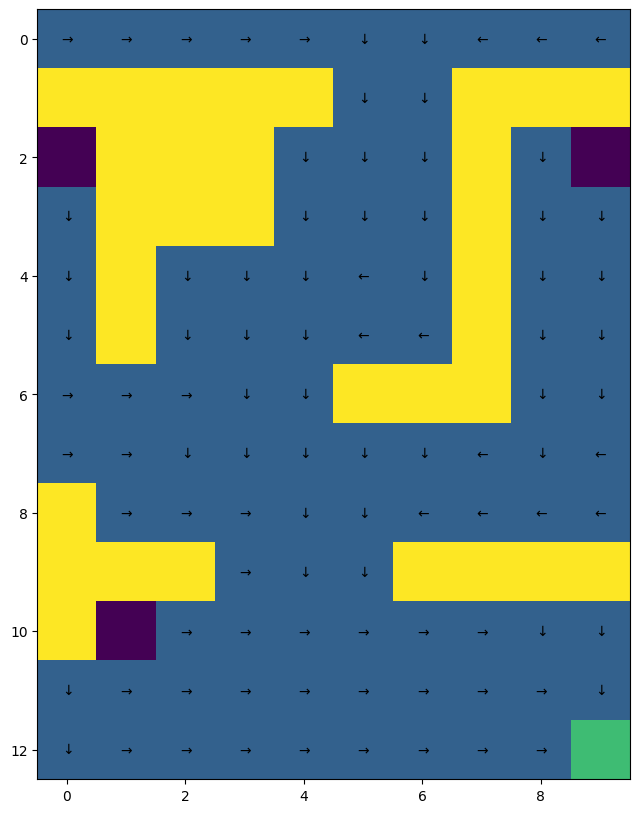
\includegraphics[width=\textwidth]{assets/mc/mc_policy.png}        
        \caption{Monte Carlo Policy}
    \end{subfigure}
    \hfill 
    \begin{subfigure}[b]{0.4\textwidth}
        \centering
        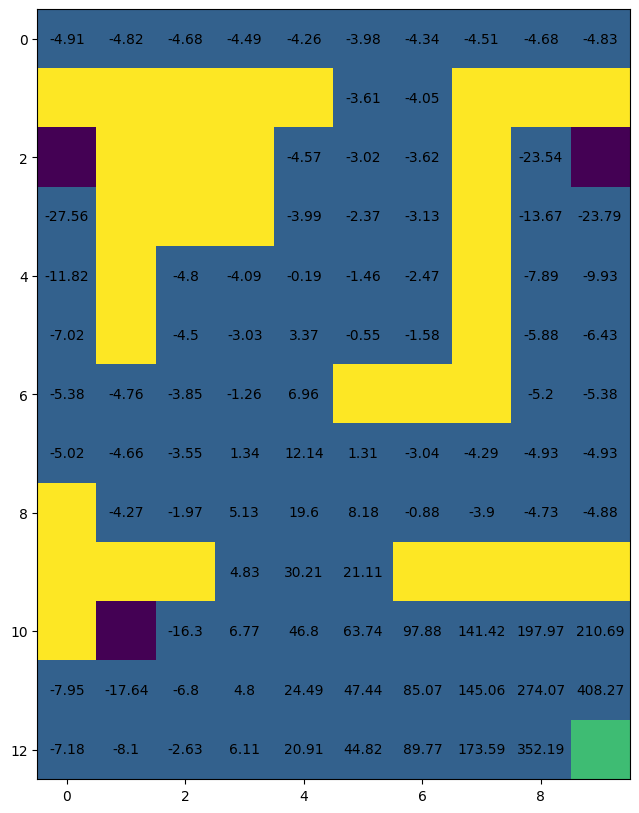
\includegraphics[width=\textwidth]{assets/mc/mc_value.png}        
        \caption{Monte Carlo Value Function}
    \end{subfigure}
    \caption*{Graphical Representations of Monte Carlo Results}
\end{figure} 

\subsection*{3}
\begin{figure}[H]
    \centering
    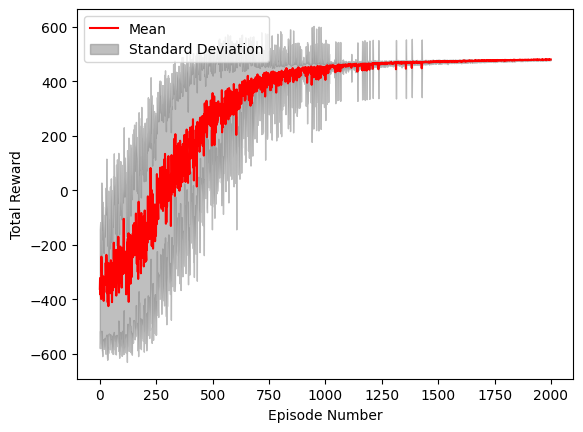
\includegraphics[width=0.8\textwidth]{assets/mc/mean_std_plot.png}
    \caption{Mean and Standard Deviation of Total Non-Discounted Sum vs Episode}
    \label{figure: total reward vs episode mc}
\end{figure} 

Figure \ref{figure: total reward vs episode mc} shows the mean
total reward and standard deviation across each episode over 2000
episodes. Inidividual runs are not shown for clarity. Note that
the total reward function approaches a limit % TODO

